%%%%%%%%%%%%%%%%%%%%%%%%%%%%%%%%%%%%%%%%%%%%%%%%%%%%%%%%%%%%%%%%%%%%%%%%
%                                                                      %
%     File: Thesis_Appendix_A.tex                                      %
%     Tex Master: Thesis.tex                                           %
%                                                                      %
%     Author: Andre C. Marta                                           %
%     Last modified :  2 Jul 2015                                      %
%                                                                      %
%%%%%%%%%%%%%%%%%%%%%%%%%%%%%%%%%%%%%%%%%%%%%%%%%%%%%%%%%%%%%%%%%%%%%%%%

\chapter{Appendix A}

\begin{table}[]
	\resizebox{\textwidth}{!}{
	\begin{tabular}{|l|l|l|l|l|}
	\hline
	\backslashbox{Security\\Level}{Operation}                  & \textbf{RSA Sign}    & \textbf{RSA Verify} & \textbf{ECDSA Sign} & \textbf{ECDSA Verify} \\ \hline
	\textbf{low}       & 20559190 (117075)    & 398584 (198)        & 14497591 (49045)    & 26839273 (50816)      \\ \hline
	\textbf{normal}    & 75738802 (317047)    & 1117868 (748)       & 29512991 (95776)    & 56260702 (162365)     \\ \hline
	\textbf{high}      & 317087210 (716961)   & 3295296 (254)       & 49150396 (82047)     & 94077150 (130275)     \\ \hline
	\textbf{very high} & 1700652764 (2283718) & 13436728 (702)      & 59732056 (441815)   & 114744021 (843861)    \\ \hline
	\end{tabular}}
	\centering \caption{\label{table:rsa-costs-all-sls} RSA and ECDSA signature creation and verification costs in number of CPU cycles. Numbers in parenthesis is the standard deviation} \end{table}
  
  \begin{table}[]
	\begin{tabular}{|l|l|l|}
	\hline
	\backslashbox{Security\\Level}{Operation}                   & \textbf{RSA Total} & \textbf{ECDSA Total} \\ \hline
	\textbf{low}       & 20957774           & 41336864             \\ \hline
	\textbf{normal}    & 76856670           & 85773693             \\ \hline
	\textbf{high}      & 320382506          & 143227546            \\ \hline
	\textbf{very high} & 1714089492         & 174476077            \\ \hline
	\end{tabular}
	\centering \caption{\label{table:rsa-costs-all-sls-total} RSA and ECDSA costs of signature creation + signature verification in number of CPU cycles}
  \end{table}
  
  \begin{table}[]
	\begin{tabular}{|l|l|l|l|}
	\hline
   \backslashbox{Security\\Level}{Opeation}                    & \textbf{RSA Sign} & \textbf{RSA Verify} & \textbf{RSA Total} \\ \hline
	\textbf{low}       & -                 & -                   & -                  \\ \hline
	\textbf{normal}    & 55179612          & 719284              & 55898896           \\ \hline
	\textbf{high}      & 241348408         & 2177428             & 243525836          \\ \hline
	\textbf{very high} & 1383565554        & 10141432            & 1393706986         \\ \hline
	\end{tabular}
	\centering \caption{\label{table:rsa-absolute-cost-increase} Absolute increase of RSA operation costs from previous security level in number of CPU cycles}
	\end{table}
  
  \begin{table}[]
  \begin{tabular}{|l|l|l|l|}
  \hline
   \backslashbox{Security\\Level}{Opeation}                  & \textbf{ECDSA Sign} & \textbf{ECDSA Verify} & \textbf{ECDSA Total} \\ \hline
  \textbf{low}       & -                   & -                     & -                    \\ \hline
  \textbf{normal}    & 15015400            & 29421429              & 44436829             \\ \hline
  \textbf{high}      & 19637405            & 37816448              & 57453853             \\ \hline
  \textbf{very high} & 10581660            & 20666871              & 31248531             \\ \hline
  \end{tabular}
  \centering \caption{\label{table:ecdsa-absolute-cost-increase} Absolute increase of ECDSA operations cost from previous security level in number of CPU cycles}
  \end{table}
  
  \begin{table}[]
	\begin{tabular}{|l|l|l|l|l|}
	\hline
	 \backslashbox{Key\\Exchange}{Security\\Level}                     & \textbf{low} & \textbf{normal} & \textbf{high} & \textbf{very high} \\ \hline
	\textbf{PSK}         & 0            & 0               & 0             & 0                  \\ \hline
	\textbf{RSA}         & 654077       & 2622235         & 5285561       & 16398134           \\ \hline
	\textbf{RSA-PSK}     & 654077       & 2622235         & 5285561       & 16398134           \\ \hline
	\textbf{ECDH-RSA}    & 1117868      & 1117868         & 1117868       & 1117868           \\ \hline
	\textbf{ECDH-ECDSA}  & 56260702     & 56260702        & 56260702      & 56260702          \\ \hline
	\textbf{ECDHE-PSK}   & 0            & 0               & 0             & 0                  \\ \hline
	\textbf{ECDHE-RSA}   & 1516452       & 2235736         & 4413164       & 14554596           \\ \hline
	\textbf{ECDHE-ECDSA} & 83099975     & 112521404       & 150337852     & 171004723          \\ \hline
	\textbf{DHE-PSK}     & 0            & 0               & 0             & 0                  \\ \hline
	\textbf{DHE-RSA}     & 1516452       & 2235736         & 4413164       & 14554596           \\ \hline
	\end{tabular}
	\centering \caption{\label{table:tls-auth-cost-client} Client authentication costs for all ciphersuites and security levels in number of CPU cycles}
	\end{table}
  
  \begin{table}[]
  \begin{tabular}{|l|l|l|l|l|}
  \hline
   \backslashbox{Key\\Exchange}{Security\\Level}                     & \textbf{low} & \textbf{normal} & \textbf{high} & \textbf{very high} \\ \hline
  \textbf{PSK}         & 0            & 0               & 0             & 0                  \\ \hline
  \textbf{RSA}         & 20362831     & 75129504        & 314975365     & 1691976601         \\ \hline
  \textbf{RSA-PSK}     & 20362831     & 75129504        & 314975365     & 1691976601         \\ \hline
  \textbf{ECDH-RSA}    & 0            & 0               & 0             & 0                  \\ \hline
  \textbf{ECDH-ECDSA}  & 0            & 0               & 0             & 0                  \\ \hline
  \textbf{ECDHE-PSK}   & 0            & 0               & 0             & 0                  \\ \hline
  \textbf{ECDHE-RSA}   & 20559190     & 75738802        & 317087210     & 1700652764         \\ \hline
  \textbf{ECDHE-ECDSA} & 14497591     & 29512991        & 49150396      & 59732056           \\ \hline
  \textbf{DHE-PSK}     & 0            & 0               & 0             & 0                  \\ \hline
  \textbf{DHE-RSA}     & 20559190     & 75738802        & 317087210     & 1700652764         \\ \hline
  \end{tabular}
	\centering \caption{\label{table:tls-auth-cost-server} Server authentication costs for all ciphersuites and security levels in number of CPU cycles}
  \end{table}
  
  \begin{table}[]
  \resizebox{\textwidth}{!}{
  \begin{tabular}{|l|l|l|l|l|}
  \hline
   \backslashbox{Security\\Level}{Opeation}                   & \textbf{ECDH Gen Keypair} & \textbf{ECDH Gen Secret} & \textbf{DH Gen Keypair} & \textbf{DH Gen Secret} \\ \hline
  \textbf{low}       & 12942518 (33356)          & 12462677 (55222)         & 10455300 (31005)        & 10279378 (27044)       \\ \hline
  \textbf{normal}    & 27483912 (94940)          & 26958612 (137745)        & 67136033 (108793)       & 66712994 (107669)      \\ \hline
  \textbf{high}      & 45900358 (65731)          & 44331330 (100040)        & 474938146 (490496)      & 473634908 (493588)     \\ \hline
  \textbf{very high} & 54449740 (487567)         & 53531554 (776984)        & 3592631108 (2792006)    & 3586324217 (2791154)   \\ \hline
  \end{tabular}}
  \centering \caption{\label{table:ecdh-dh-costs-all-sls} ECDH and DH costs for all security levels in number of CPU cycles. Numbers in parenthesis are the standard deviation.}
  \end{table}
  
  \begin{table}[]
  \begin{tabular}{|l|l|l|}
  \hline
   \backslashbox{Security\\Level}{Operation}                   & \textbf{ECDH Total} & \textbf{DH Total} \\ \hline
  \textbf{low}       & 25405195            & 20734678          \\ \hline
  \textbf{normal}    & 54442524            & 133849027         \\ \hline
  \textbf{high}      & 90231688            & 948573054         \\ \hline
  \textbf{very high} & 90231688            & 7178955325        \\ \hline
  \end{tabular}
  \centering \caption{\label{table:ecdh-dh-costs-total-all-sls} ECDH and DH costs of the sum of keypair and shared secret generation in number of CPU cycles}
  \end{table}
  
  \begin{table}[]
  \begin{tabular}{|l|l|l|l|}
  \hline
   \backslashbox{Security\\Level}{Operation}                   & \textbf{ECDH Gen Keypair} & \textbf{ECDH Gen Shared} & \textbf{ECDH Total} \\ \hline
  \textbf{low}       & -                         & -                        & -                   \\ \hline
  \textbf{normal}    & 14541394                  & 14495935                 & 29037329            \\ \hline
  \textbf{high}      & 18416446                  & 17372718                 & 35789164            \\ \hline
  \textbf{very high} & 8549382                   & 9200224                  & 17749606            \\ \hline
  \end{tabular}
  \centering \caption{\label{table:ecdh-absolute-cost-increase} Absolute increase of ECDH operation costs from previous security level in number of CPU cycles}
  \end{table}
  
  \begin{table}[]
	  \begin{tabular}{|l|l|l|l|}
	  \hline
	   \backslashbox{Security\\ Level}{Operation}                   & \textbf{DH Gen Keypair} & \textbf{DH Gen Shared} & \textbf{DH Total} \\ \hline
	  \textbf{low}       & -                       & -                      & -                 \\ \hline
	  \textbf{normal}    & 56680733                & 56433616               & 113114349         \\ \hline
	  \textbf{high}      & 407802113               & 406921914              & 814724027         \\ \hline
	  \textbf{very high} & 3117692962              & 3112689309             & 6230382271        \\ \hline
	  \end{tabular}
	  \centering \caption{\label{table:dh-absolute-cost-increase} Absolute increase of DH operation costs from previous security level in number of CPU cycles}
  \end{table}
  
  \begin{table}[]
  \begin{tabular}{|l|l|l|l|l|}
  \hline
   \backslashbox{Key\\Exchange}{Security\\Level}                                           & \textbf{low}                    & \textbf{normal}                 & \textbf{high}                   & \textbf{very high}               \\ \hline
  \textbf{PSK}                               & 0                               & 0                               & 0                               & 0                                \\ \hline
  \textbf{RSA-PSK}                           & 0                               & 0                               & 0                               & 0                                \\ \hline
  \textbf{RSA}                               & 0                               & 0                               & 0                               & 0                                \\ \hline
  \rowcolor[HTML]{9B9B9B}
  {\color[HTML]{333333} \textbf{ECDH-RSA}}   & {\color[HTML]{333333} 25405195} & {\color[HTML]{333333} 54442524} & {\color[HTML]{333333} 90231688} & {\color[HTML]{333333} 107981294} \\ \hline
  \rowcolor[HTML]{9B9B9B}
  {\color[HTML]{333333} \textbf{ECDH-ECDSA}} & {\color[HTML]{333333} 25405195} & {\color[HTML]{333333} 54442524} & {\color[HTML]{333333} 90231688} & {\color[HTML]{333333} 107981294} \\ \hline
  \textbf{ECDHE-PSK}                         & 25405195                        & 54442524                        & 90231688                        & 107981294                        \\ \hline
  \textbf{ECDHE-RSA}                         & 25405195                        & 54442524                        & 90231688                        & 107981294                        \\ \hline
  \textbf{ECDHE-ECDSA}                       & 25405195                        & 54442524                        & 90231688                        & 107981294                        \\ \hline
  \textbf{DHE-PSK}                           & 20734678                        & 133849027                       & 948573054                        & 7178955325                        \\ \hline
  \textbf{DHE-RSA}                           & 25405195                        & 133849027                        & 948573054                        & 7178955325                        \\ \hline
  \end{tabular}
  \centering \caption{\label{table:pfs-cost-client} \gls{pfs} and \textit{ECDH} key exchange cost for the client in number of CPU cycles}
  \end{table}
  
  \begin{table}[]
  \begin{tabular}{|l|l|l|l|l|}
  \hline
   \backslashbox{Key\\Exchange}{Security\\Level}                                           & \textbf{low}                    & \textbf{normal}                 & \textbf{high}                   & \textbf{very high}              \\ \hline
  \textbf{PSK}                               & 0                               & 0                               & 0                               & 0                               \\ \hline
  \textbf{RSA-PSK}                           & 0                               & 0                               & 0                               & 0                               \\ \hline
  \textbf{RSA}                               & 0                               & 0                               & 0                               & 0                               \\ \hline
  \rowcolor[HTML]{9B9B9B}
  {\color[HTML]{333333} \textbf{ECDH-RSA}}   & {\color[HTML]{333333} 12462677} & {\color[HTML]{333333} 26958612} & {\color[HTML]{333333} 44331330} & {\color[HTML]{333333} 53531554} \\ \hline
  \rowcolor[HTML]{9B9B9B}
  {\color[HTML]{333333} \textbf{ECDH-ECDSA}} & {\color[HTML]{333333} 12462677} & {\color[HTML]{333333} 26958612} & {\color[HTML]{333333} 44331330} & {\color[HTML]{333333} 53531554} \\ \hline
  \textbf{ECDHE-PSK}                         & 25405195                        & 54442524                        & 90231688                        & 107981294                       \\ \hline
  \textbf{ECDHE-RSA}                         & 25405195                        & 54442524                        & 90231688                        & 107981294                       \\ \hline
  \textbf{ECDHE-ECDSA}                       & 25405195                        & 54442524                        & 90231688                        & 107981294                       \\ \hline
  \textbf{DHE-PSK}                           & 20734678                        & 133849027                       & 948573054                        & 7178955325                       \\ \hline
  \textbf{DHE-RSA}                           & 20734678                        & 133849027                       & 948573054                        & 7178955325                       \\ \hline
  \end{tabular}
  \centering \caption{\label{table:pfs-cost-server} \gls{pfs} and \textit{ECDH} key exchange cost for the server in number of CPU cycles}
  \end{table}
  
  \begin{table}[]
	\resizebox{\textwidth}{!}{
	\begin{tabular}{|l|l|l|l|l|}
	\hline
	 \backslashbox{Key\\Exchange}{Security\\Level}                     & \textbf{low}      & \textbf{normal}    & \textbf{high}      & \textbf{very high}   \\ \hline
	\textbf{PSK}         & 1354543 (51058)   & 1353865 (51289)    & 1355005 (51004)    & 1354829 (51043)      \\ \hline
	\textbf{RSA-PSK}     & 3536763 (71446)   & 4543238 (76038)    & 7293473 (84814)    & 18578392 (103341)    \\ \hline
	\textbf{RSA}         & 3556430 (59010)   & 4558935 (68078)    & 7309587 (71844)    & 18608492 (82623)     \\ \hline
	\textbf{ECDH-RSA}    & 28433250 (97731)  & 57412269 (122298)  & 93325335 (102107)  & 111532116 (623350)   \\ \hline
	\textbf{ECDH-ECDSA}  & 83731926 (78435)  & 112585306 (128327) & 148415289 (126285) & 166815336 (554471)   \\ \hline
	\textbf{ECDHE-PSK}   & 26819362 (68991)  & 55805138 (138561)  & 91713096 (142807)  & 109203285 (813689)   \\ \hline
	\textbf{ECDHE-RSA}   & 28862986 (105477) & 58608367 (214574)  & 96730901 (93708)   & 124773055 (696488)   \\ \hline
	\textbf{ECDHE-ECDSA} & 110524836 (93990) & 168954007 (267635) & 242501399 (149155) & 280626510 (1071418)  \\ \hline
	\textbf{DHE-PSK}     & 22189619 (55603)  & 135442518 (309751) & 950212732 (787892) & 7181764421 (5195398) \\ \hline
	\textbf{DHE-RSA}     & 24250886 (94421)  & 138197524 (198704) & 955840114 (861069) & 7196088947 (6405987) \\ \hline
	\end{tabular}}
	\centering \caption{\label{table:client-hs-cost-all-sls} Handshake costs for the client in number of CPU cycles. Numbers in parenthesis are the standard deviation}
	\end{table}
  
	\begin{table}[]
		\resizebox{\textwidth}{!}{
  \begin{tabular}{|l|l|l|l|l|}
  \hline
   \backslashbox{Key\\Exchange}{Security\\Level}                     & \textbf{low}      & \textbf{normal}    & \textbf{high}       & \textbf{very high}   \\ \hline
  \textbf{PSK}         & 1380956 (50888)   & 1382849 (50737)    & 1381497 (50891)     & 1382002 (50903)      \\ \hline
  \textbf{RSA-PSK}     & 22515609 (111975) & 77368868 (275574)  & 317389619 (662953)  & 1694178055 (2427763) \\ \hline
  \textbf{RSA}         & 22456180 (121140) & 77260738 (239418)  & 317196961 (698637)  & 1694747500 (1705523) \\ \hline
  \textbf{ECDH-RSA}    & 14534087 (49806)  & 29154666 (127699)  & 46480720 (107771)   & 55636527 (576001)    \\ \hline
  \textbf{ECDH-ECDSA}  & 14521154 (58001)  & 29094320 (111114)  & 46390603 (132250)   & 55927921 (688074)    \\ \hline
  \textbf{ECDHE-PSK}   & 26869449 (110405) & 56020895 (147825)  & 91773474 (94656)    & 109500050 (905013)   \\ \hline
  \textbf{ECDHE-RSA}   & 48164890 (126885) & 132433386 (379327) & 409652623 (951326)  & 1810563620 (3011341) \\ \hline
  \textbf{ECDHE-ECDSA} & 41984222 (82371)  & 86096716 (192885)  & 141506181 (147013)  & 169996896 (1051307)  \\ \hline
  \textbf{DHE-PSK}     & 22308029 (76182)  & 135535409 (232955) & 950691653 (1289706) & 7181243788 (5402427) \\ \hline
  \textbf{DHE-RSA}     & 43602094 (154553) & 212251542 (364611) & 1268235354 (857921) & 8883866054 (5993186) \\ \hline
  \end{tabular}}
	\centering \centering \caption{\label{table:server-hs-cost-all-sls} Handshake costs for the server in number of CPU cycles. Numbers in parenthesis are the standard deviation}
  \end{table}
  
  
	  \begin{table}[]
		\begin{tabular}{|l|l|l|l|l|}
		\hline
		\backslashbox{Security\\Level}{Operation}                 & \textbf{RSA Sign} & \textbf{RSA Verify} & \textbf{ECDSA Sign} & \textbf{ECSDA Verify} \\ \hline
		\textbf{low}       & 11355 (138)       & 293 (5)             & 8487 (2010)         & 14219 (175)           \\ \hline
		\textbf{normal}    & 41672 (342)       & 747 (8)             & 16130 (441)         & 30750 (246)           \\ \hline
		\textbf{high}      & 176255 (997)      & 2096 (15)           & 26961 (221)         & 51457 (272)           \\ \hline
		\textbf{very high} & 939928 (3238)     & 7704 (33)           & 34246 (334)         & 65877 (549)           \\ \hline
		\end{tabular}
		\caption{RSA and ECDSA signature creation and verification costs in microseconds. Numbers in parenthesis is the standard deviation}
		\label{table:rsa-ecdsa-costs-papi}
		\end{table}
  
		\begin{table}[]
		  \begin{tabular}{|l|l|l|l|l|}
		  \hline
		   \backslashbox{Key\\Exchange}{Security\\Level}                    & \textbf{low} & \textbf{normal} & \textbf{high} & \textbf{very high} \\ \hline
		  \textbf{PSK}         & 0            & 0               & 0             & 0                  \\ \hline
		  \textbf{ECDHE-PSK}   & 0            & 0               & 0             & 0                  \\ \hline
		  \textbf{DHE-PSK}     & 0            & 0               & 0             & 0                  \\ \hline
		  \textbf{ECDH-RSA}    & 683 (9)       & 683 (6)          & 678 (11)       & 682 (6)             \\ \hline
		  \textbf{ECDHE-RSA}   & 1014 (120)    & 1446 (115)       & 2805 (122)     & 8406 (123)          \\ \hline
		  \textbf{DHE-RSA}     & 1000 (119)    & 1439 (103)       & 2798 (119)     & 8388 (126)          \\ \hline
		  \textbf{RSA}         & 1061 (14)     & 1712 (23)        & 3436 (25)      & 9806 (55)           \\ \hline
		  \textbf{RSA-PSK}     & 1060 (9)      & 1710 (22)        & 3438 (27)      & 9804 (51)           \\ \hline
		  \textbf{ECDH-ECDSA}  & 30722 (272)   & 30847 (243)      & 30631 (210)    & 30765 (363)         \\ \hline
		  \textbf{ECDHE-ECDSA} & 46368 (3693)  & 62989 (3636)     & 83322 (3383)   & 97615 (2980)        \\ \hline
		  \end{tabular}
		  \caption{Client authentication costs for all ciphersuites and security levels in microseconds}
		  \label{table:papi-cli-auth-cost}
		  \end{table}
  
		  \begin{table}[]
			\begin{tabular}{|l|l|l|l|l|}
			\hline
			\backslashbox{Key\\Exchange}{Security\\Level}                    & \textbf{low} & \textbf{normal} & \textbf{high} & \textbf{very high} \\ \hline
			\textbf{PSK}         & 0            & 0               & 0             & 0                  \\ \hline
			\textbf{ECDHE-PSK}   & 0            & 0               & 0             & 0                  \\ \hline
			\textbf{DHE-PSK}     & 0            & 0               & 0             & 0                  \\ \hline
			\textbf{ECDH-RSA}    & 0            & 0               & 0             & 0                  \\ \hline
			\textbf{ECDHE-RSA}   & 11342 (138)   & 41659 (342)      & 176241 (997)   & 939913 (3238)       \\ \hline
			\textbf{DHE-RSA}     & 11329 (135)   & 41689 (694)      & 176192 (1197)  & 939929 (3698)       \\ \hline
			\textbf{RSA}         & 11286 (178)   & 41403 (411)      & 175097 (1089)  & 936521 (3356)       \\ \hline
			\textbf{RSA-PSK}     & 11259 (156)   & 41372 (348)      & 175107 (1114)  & 935820 (3347)       \\ \hline
			\textbf{ECDH-ECDSA}  & 0            & 0               & 0             & 0                  \\ \hline
			\textbf{ECDHE-ECDSA} & 8474 (2008)   & 16117 (440)      & 26947 (221)    & 34231 (334)         \\ \hline
			\end{tabular}
			\caption{Server authentication costs for all ciphersuites and security levels in microseconds}
			\label{table:server-auth-costs-papi}
			\end{table}
  
			\begin{table}[]
				\resizebox{\textwidth}{!}{
			  \begin{tabular}{|l|l|l|l|l|}
			  \hline
			   \backslashbox{Security\\Level}{Operation}                  & \textbf{ECDH Gen Keypair} & \textbf{ECDH Gen Shared} & \textbf{DH Gen Keypair} & \textbf{DH Gen Shared} \\ \hline
			  \textbf{low}       & 6884 (45)                 & 6593 (67)                 & 6028 (127)               & 5878 (171)              \\ \hline
			  \textbf{normal}    & 15049 (158)                & 14693 (131)               & 37422 (325)              & 36969 (275)             \\ \hline
			  \textbf{high}      & 25139 (305)                & 24297 (187)               & 263498 (843)             & 262432 (927)            \\ \hline
			  \textbf{very high} & 31270 (342)                & 30830 (455)               & 1959755 (3784)           & 1955550 (4082)          \\ \hline
			  \end{tabular}}
			  \caption{ECDH  and  DH  costs  for  all  security  levels  in  microseconds.  Numbers  in parenthesis are the standard deviation}
			  \label{table:papi-ecd-dh-costs}
			  \end{table}
  
			  \begin{table}[]
				\begin{tabular}{|l|l|l|l|l|}
				\hline
				 \backslashbox{Key\\Exchange}{Security\\Level}                    & \textbf{low} & \textbf{normal} & \textbf{high} & \textbf{very high} \\ \hline
				\textbf{PSK}         & 1024 (97)    & 1038 (95)        & 1013 (82)      & 1028 (96)           \\ \hline
				\textbf{RSA-PSK}     & 2531 (121)    & 3204 (103)       & 4954 (125)     & 11388 (136)         \\ \hline
				\textbf{RSA}         & 2537 (132)    & 3202 (108)       & 4948 (124)     & 11387 (140)         \\ \hline
				\textbf{ECDH-RSA}    & 15709 (187)  & 31966 (309)      & 51570 (389)    & 64849 (538)         \\ \hline
				\textbf{ECDH-ECDSA}  & 45665 (384)   & 61924 (386)      & 81463 (385)    & 94748 (651)         \\ \hline
				\textbf{ECDHE-PSK}   & 14605 (148)  & 30893 (264)      & 50525 (438)    & 63219 (641)         \\ \hline
				\textbf{ECDHE-RSA}   & 16138 (344)  & 32831 (371)      & 53778 (397)    & 72269 (761)         \\ \hline
				\textbf{ECDHE-ECDSA} & 61255 (3776)  & 94156 (3729)     & 134140 (3479)  & 161190 (3168)       \\ \hline
				\textbf{DHE-PSK}     & 13086 (283)  & 75520 (426)      & 527114 (1356)  & 3916656 (6127)      \\ \hline
				\textbf{DHE-RSA}     & 14607(382)   & 77476 (521)      & 531919 (1841)  & 3930292 (6979)      \\ \hline
				\end{tabular}
				\caption{Handshake costs for the client in microseconds. Numbers in parenthesis are the standard deviation}
				\label{table:hs-costs-cli-papi}
				\end{table}
  
				\begin{table}[]
				  \begin{tabular}{|l|l|l|l|l|}
				  \hline
				   \backslashbox{Key\\Exchange}{Security\\Level}                    & \textbf{low} & \textbf{normal} & \textbf{high} & \textbf{very high} \\ \hline
				  \textbf{PSK}         & 1029 (90)     & 1048 (89)        & 1021 (76)      & 1033 (90)           \\ \hline
				  \textbf{RSA-PSK}     & 12668 (166)   & 42809 (355)      & 176543 (1118)  & 937388 (3348)       \\ \hline
				  \textbf{RSA}         & 12685 (188)   & 42828 (414)      & 176527 (1091)  & 938082 (3359)       \\ \hline
				  \textbf{ECDH-RSA}    & 8129 (180)    & 16187 (322)      & 26366 (2121)   & 32412 (483)         \\ \hline
				  \textbf{ECDH-ECDSA}  & 8137 (200)    & 16160 (170)      & 25842 (233)    & 32350 (473)         \\ \hline
				  \textbf{ECDHE-PSK}   & 14769 (256)   & 30919 (291)      & 50787 (321)    & 63563 (548)         \\ \hline
				  \textbf{ECDHE-RSA}   & 26628 (485)   & 73075 (591)      & 227665 (1194)  & 1004212 (3334)      \\ \hline
				  \textbf{ECDHE-ECDSA} & 24408 (4163)  & 48707 (3657)     & 79316 (3321)   & 98991 (2870)        \\ \hline
				  \textbf{DHE-PSK}     & 13139 (147)   & 75741 (423)      & 527735 (1390)  & 3925059 (9696)      \\ \hline
				  \textbf{DHE-RSA}     & 24964 (365)   & 117961 (1399)    & 704677 (1918)  & 4864588 (13183)     \\ \hline
				  \end{tabular}
				  \caption{Handshake costs for the server in microseconds. Numbers in parenthesis are the standard deviation}
				  \label{table:server-hs-costs-papi}
				  \end{table}
				  
				  \begin{figure}
					\centering
					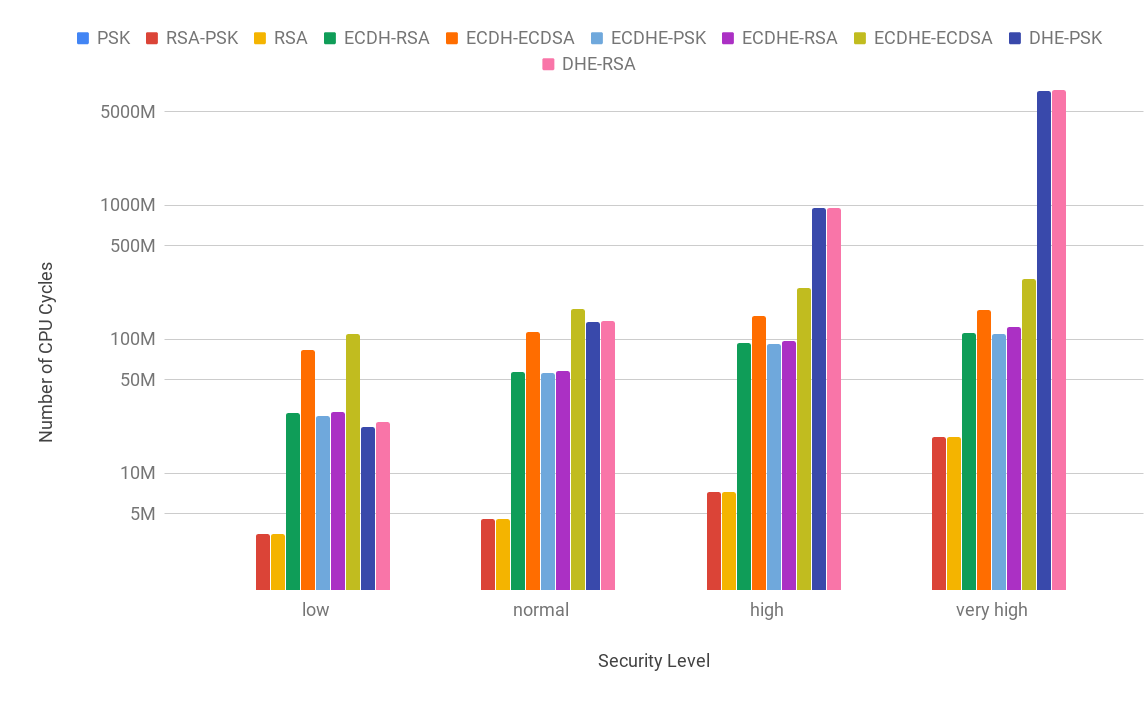
\includegraphics[width=1.0\textwidth]{img/chart-20.png}
					\centering \caption{Handshake cost for the client in estimated number of CPU cycles (logarithmic scale). This representation 
					of the Handshake costs assists in visual comparison between the results obtained with \gls{papi} and \textit{valgrind}.}
					\label{fig:a-cli}
				  \end{figure}

				  \begin{figure}
					\centering
					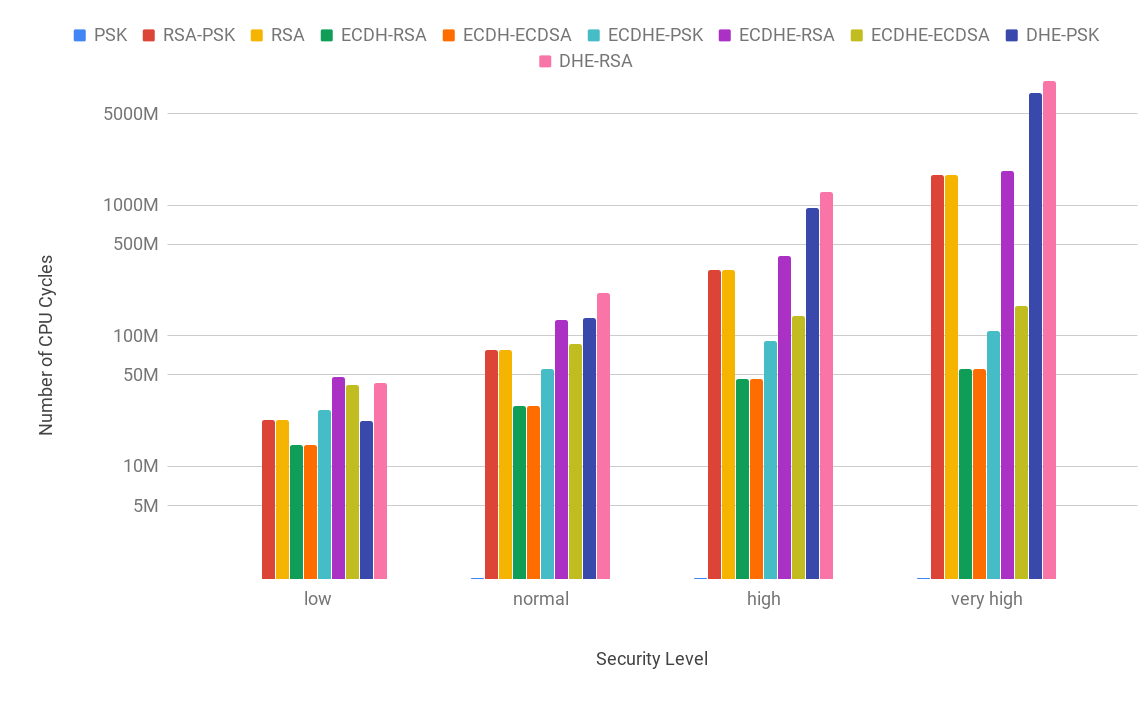
\includegraphics[width=1.0\textwidth]{img/chart-21.png}
					\centering \caption{Handshake cost for the client in estimated number of CPU cycles (logarithmic scale). This representation 
					of the Handshake costs assists in visual comparison between the results obtained with \gls{papi} and \textit{valgrind}.}
					\label{fig:a-srv}
				  \end{figure}

				  \begin{figure}
					\centering
					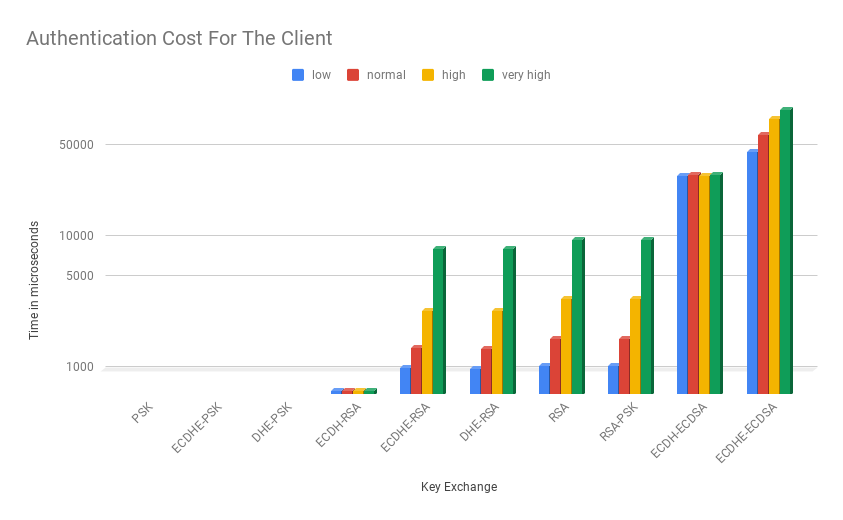
\includegraphics[width=1.0\textwidth]{img/papi-client-auth-cost.png}
					\centering \caption{Authentication cost for the client in microseconds (logarithmic scale)}
					\label{af:1}
				  \end{figure}
  
				  \begin{figure}
					\centering
					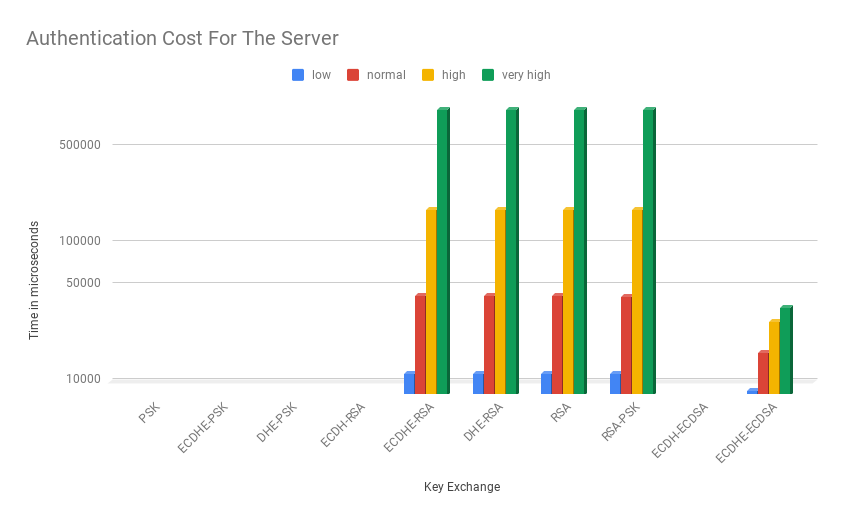
\includegraphics[width=1.0\textwidth]{img/papi-server-auth-cost.png}
					\centering \caption{Authentication cost for the server in microseconds (logarithmic scale)}
					\label{af:2}
				  \end{figure}
  
				  \begin{figure}
					\centering
					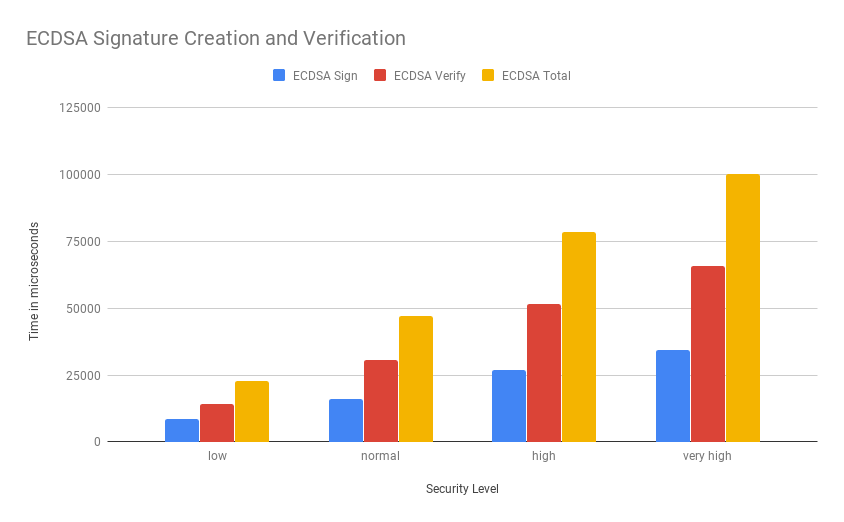
\includegraphics[width=1.0\textwidth]{img/papi-ecdsa-sign-verify.png}
					\centering \caption{ECDSA signature creation and verification costs in microseconds}
					\label{af:3}
				  \end{figure}
  
				  \begin{figure}
					\centering
					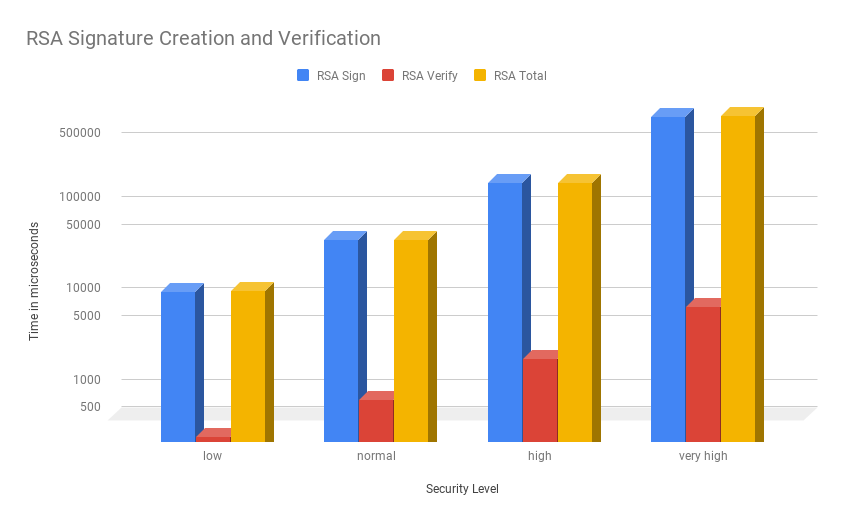
\includegraphics[width=1.0\textwidth]{img/papi-rsa-sign-verify.png}
					\centering \caption{RSA signature creation and verification costs in microseconds (logarithmic scale)}
					\label{af:4}
				  \end{figure}
  
				  \begin{figure}
					\centering
					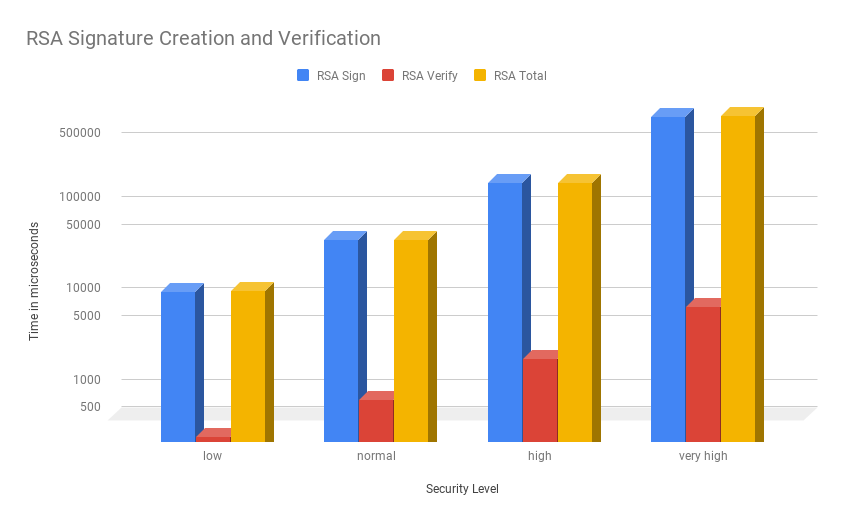
\includegraphics[width=1.0\textwidth]{img/papi-rsa-sign-verify.png}
					\centering \caption{RSA encryption and decryption costs in microseconds (logarithmic scale)}
					\label{af:5}
				  \end{figure}
  
				  \begin{figure}
					\centering
					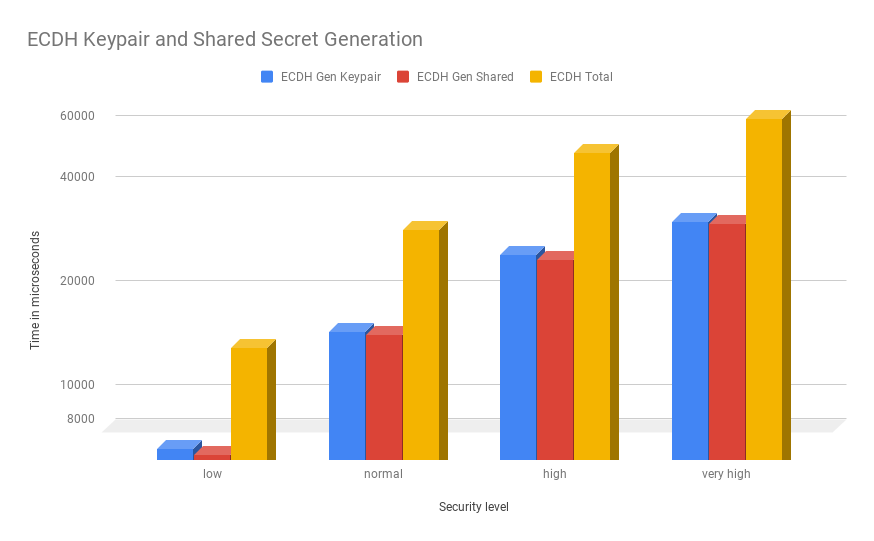
\includegraphics[width=1.0\textwidth]{img/papi-ecdh-cost.png}
					\centering \caption{ECDH keypair and shared secret generation costs in microseconds (logarithmic scale)}
					\label{af:6}
				  \end{figure}
  
				  \begin{figure}
					\centering
					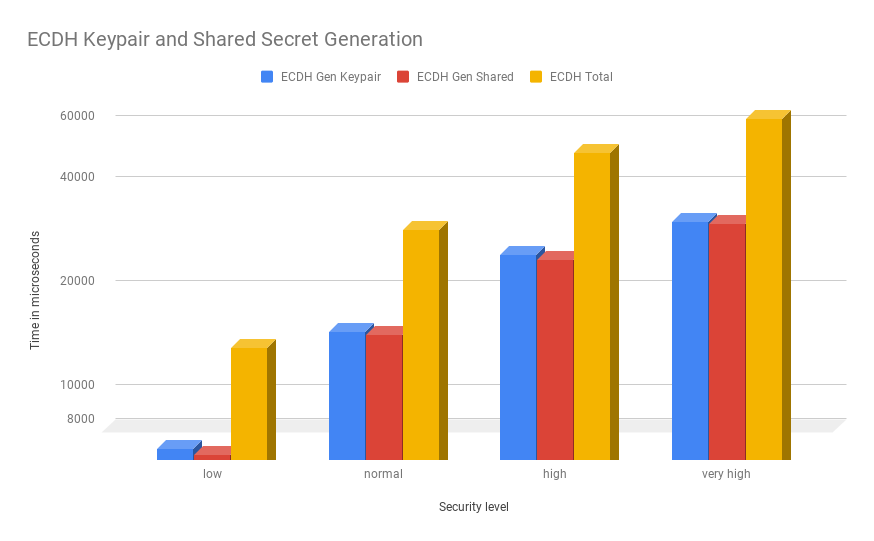
\includegraphics[width=1.0\textwidth]{img/papi-ecdh-cost.png}
					\centering \caption{DH keypair and shared secret generation costs in microseconds (logarithmic scale)}
					\label{af:7}
				  \end{figure}
  